\chapter{LITERATURE REVIEW}
\label{chap:lit}

\section{Overview}
There is plenty of work in graph and optmization literature to learn graphs from data. \cite{friedman2008sparse} proposed Graphical Lasso (GLasso henceforth) to learn sparse graphs by imposing $l1$-norm penalty on the precision matrix. Solving the following optimization problem to obtain the positive semi-definite precision matrix $\Theta$:
$$\min _{\Theta \succeq 0} \operatorname{tr}(S \Theta)-\log \operatorname{det}(\Theta)+\lambda\|\Theta\|_{1}$$
, where $\lambda$ is the regularization parameter. 
\cite{kumar2019structured, kumar2020unified} provided a unified approach for learning a large class of structured graph families, e.g., multi-component, bipartite, regular, etc. Their proposed algorithm learns graphs under the given structural constraints of the graph structure. These structural constraints are converted into the spectral constraints of graph and then imposed on either the laplacian matrix (SGL henceforth) or the adjacency matrix (SGA henceforth) or both of them (SGLA henceforth). The following optimization objective is solved to learn the graph:
$$\begin{array}{ll}
\underset{\Theta}{\operatorname{maximize}} & \log \operatorname{gdet}(\Theta)-\operatorname{tr}(\Theta S)-\alpha h(\Theta) \\
\text { subject to } & \Theta \in \mathcal{S}_{\Theta}, \lambda(\mathcal{T}(\Theta)) \in \mathcal{S}_{\mathcal{T}}
\end{array}$$
, where gdet (·) is the generalized determinant defined as the non-zero eigenvalues product, $\mathcal{S}_{\Theta}$ encodes the typical constraints of a Laplacian matrix , $\lambda(\mathcal{T}(\Theta))$ is the vector containing the eigenvalues of matrix $\mathcal{T}(\Theta)$, $\mathcal{T}$ (·) is the transformation matrix to consider the eigenvalues of different graph matrices, and $\mathcal{S}_{\mathcal{T}}$ allows to include spectral constraints in the eigenvalues.
%TODO: improve above para
The main idea of structured graph learning is that structural properties of graphs are encoded in their spectral properties. Fig~\ref{fig:kcomp-eig} shows a 3-component graph and the distribution of corresponding eigenvalues of the Laplacian matrix with first three eigenvalues zero. For a k-component graph, first k of its eigenvalues are zero. Similarly, Fig~\ref{fig:bipartite-eig} shows a bipartite graph and its corresponding eigenvalues which are symmetric around origin.
\begin{center}
	\begin{figure}[htpb]
		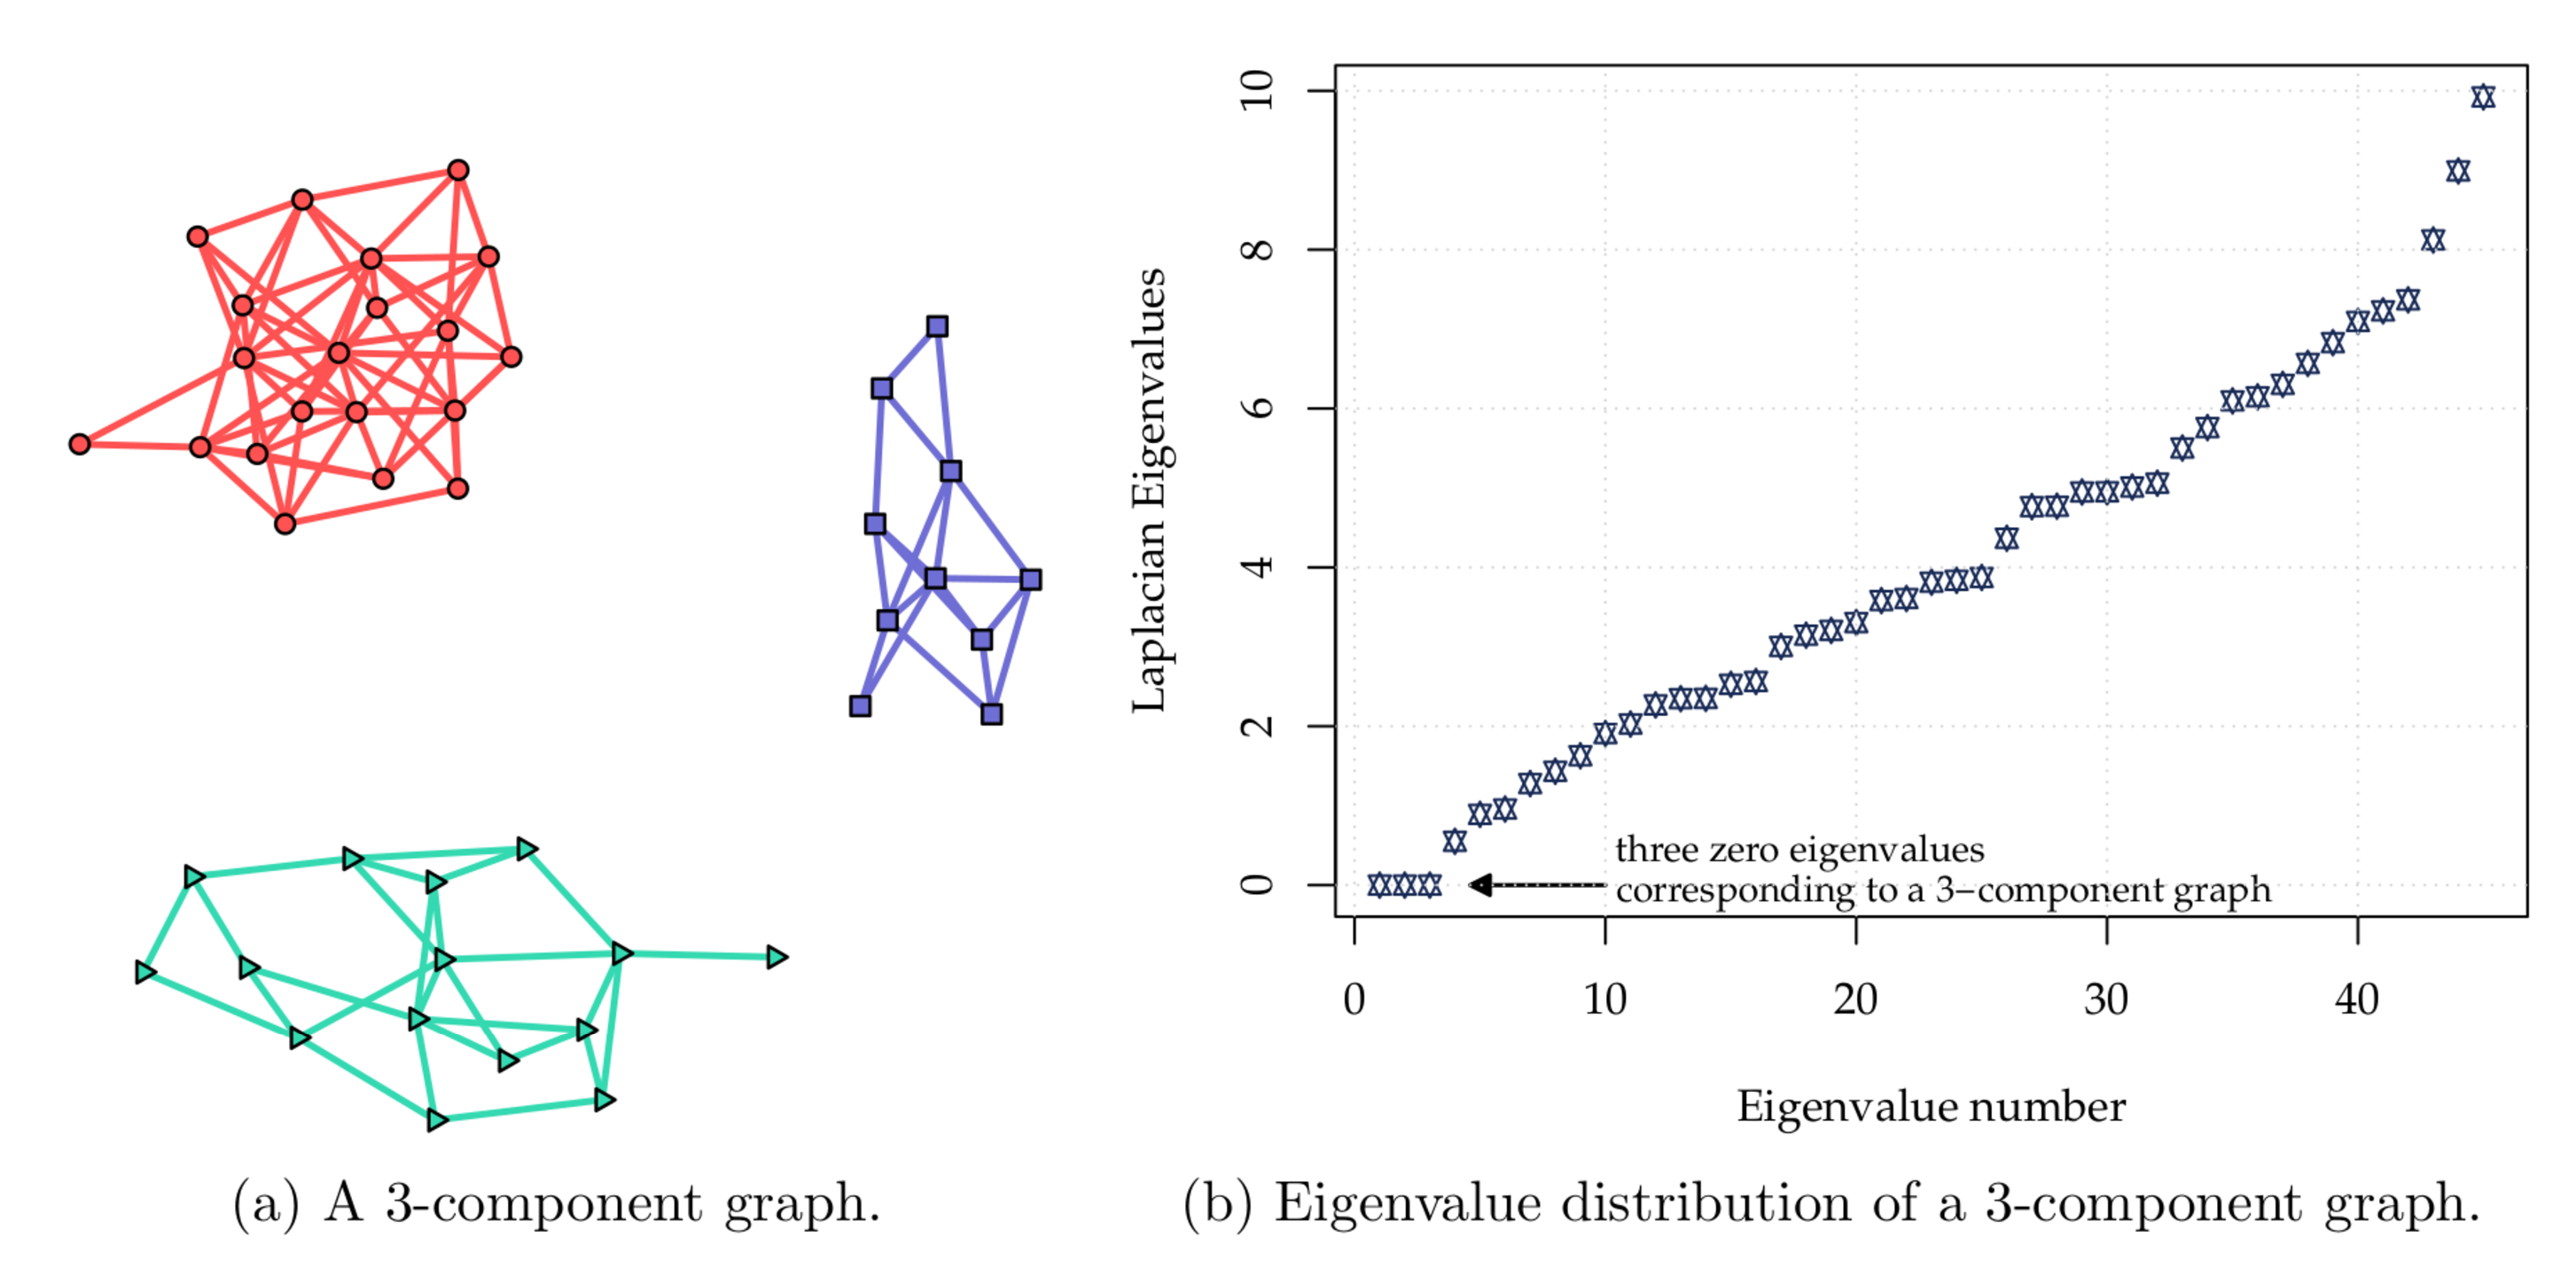
\includegraphics[scale=0.3]{Pictures/kcomp.eps}
		\caption{3-component graph and its eigenvalue distribution. Image src: \cite{kumar2020unified}  }
		\label{fig:kcomp-eig}
	\end{figure}
\end{center}

\begin{center}
	\begin{figure}[htpb]
		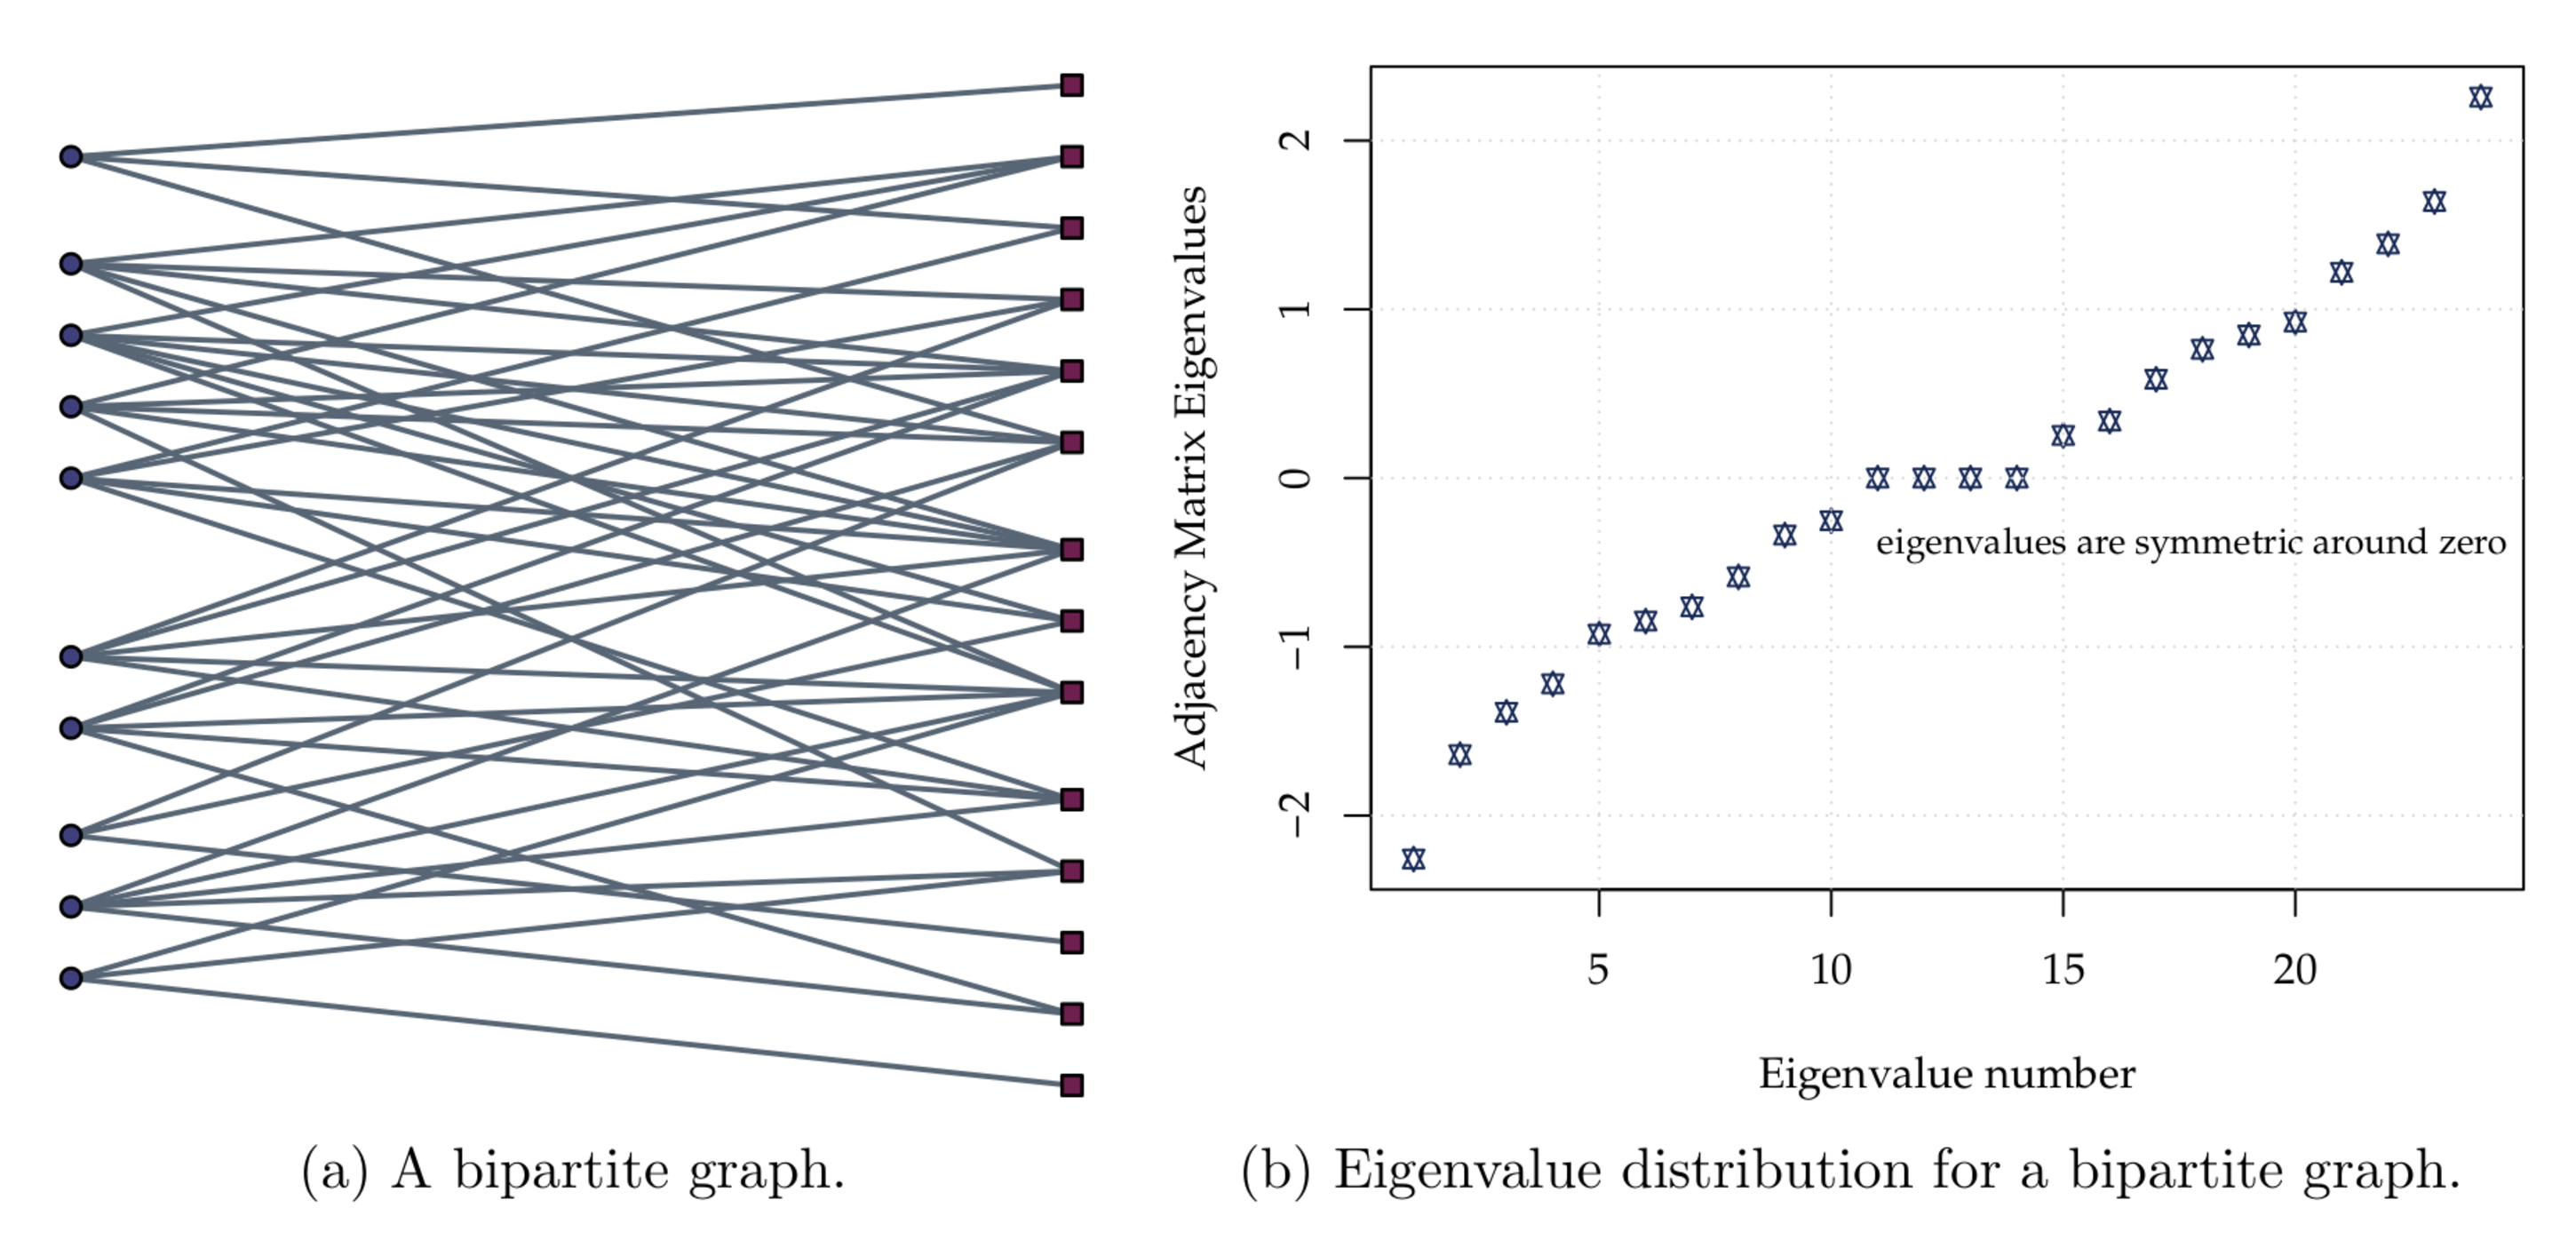
\includegraphics[scale=0.3]{Pictures/bipartite.eps}
		\caption{Bipartite graph and its eigenvalue distribution. Image src: \cite{kumar2020unified}  }
		\label{fig:bipartite-eig}
	\end{figure}
\end{center}

Therefore, the SGL/SGA/SGLA algorithms requires knowledge of the graph structure \textit{a priori}, based on which it can learn the graph by incorporating the spectral constraints in the optimization objective. However, in many modern applications, e.g., network medicine, gene regulatory networks, we do not have a prior information of the type of graph structure suitable for that particular data. In such cases structure identifiability from data becomes very crucial for building a graph-based application. Thus, before learning a graph it become imperative to identify best suitable type of graph structure for that data. This issue has not been explored in the literature, which will be the focus of our work.  We envision that this problem can be tackled by integrating model selection, degree of freedom and conditional measure frameworks  within the algorithmic framework developed by \cite{kumar2020unified}.

The previous attempts of graph model selection in GGMs tries to choose the best graph at the sparsity level \citep{lartigue2020gaussian} or to enforce connectedness in the graph \citep{foygel2010extended}.  No prior work for model selection of graph type has been done earlier to the best of our knowledge. Our proposed formulation will allow us to directly learn the graph from data without requiring any structural (or any other) constraints.
